\input{../utils/preamble}
\createdgmtitle{13}

\usepackage{tikz}

\usetikzlibrary{arrows,shapes,positioning,shadows,trees}
%--------------------------------------------------------------------------------
\begin{document}
%--------------------------------------------------------------------------------
\begin{frame}[noframenumbering,plain]
%\thispagestyle{empty}
\titlepage
\end{frame}
%=======
\begin{frame}{Recap of previous lecture}
	\begin{block}{ELBO of gaussian diffusion model}
		\vspace{-0.7cm}
		\begin{multline*}
			\cL(q, \btheta) =  {\color{olive}\bbE_{q(\bx_1 | \bx_0)} \log p(\bx_0 | \bx_1, \btheta)} - {\color{violet}KL\bigl(q(\bx_T | \bx_0) || p(\bx_T)\bigr)} - \\
			- \sum_{t=2}^T  \underbrace{ \bbE_{q(\bx_t | \bx_0)}KL \bigl(q(\bx_{t-1} | \bx_t, \bx_0) || p(\bx_{t - 1} | \bx_t, \btheta )\bigr)}_{\cL_t}
		\end{multline*}
		\vspace{-1.0cm}
	\end{block}
	\begin{align*}
		q(\bx_{t-1} | \bx_t, \bx_0) &= \cN(\bx_{t-1} | \tilde{\bmu}_t(\bx_t, \bx_0), \tilde{\beta}_t \bI), \\
		p(\bx_{t - 1} | \bx_t, \btheta) &= \cN \bigl(\bx_{t - 1} | \bmu_{\btheta}(\bx_t, t), {\color{violet}\bsigma_{\btheta}^2(\bx_t, t)}\bigr)
	\end{align*}
	Our assumption:	${\color{violet}\bsigma_{\btheta}^2(\bx_t, t) = \tilde{\beta}_t \bI}$.
	\[
		\cL_t = \bbE_{q(\bx_t | \bx_0)} \left[\frac{1}{2\tilde{\beta}_t} \bigl\| \tilde{\bmu}_t(\bx_t, \bx_0) - \bmu_{\btheta}(\bx_t, t) \bigr\|^2  \right]
	\]
	\myfootnotewithlink{https://arxiv.org/abs/2006.11239}{Ho J. Denoising Diffusion Probabilistic Models, 2020}
\end{frame}
%=======
\begin{frame}{Recap of previous lecture}
	\vspace{-0.3cm}
	\[
		\cL_t = \bbE_{\color{violet}q(\bx_t | \bx_0)} \left[ {\color{olive}\frac{1}{2\tilde{\beta}_t}} \bigl\| \tilde{\bmu}_t(\bx_t, \bx_0) - \bmu_{\btheta}(\bx_t, t) \bigr\|^2  \right]
	\]
	\vspace{-0.3cm}
	\begin{block}{Reparametrization}
		\vspace{-0.7cm}
		\begin{align*}
			\tilde{\bmu}_t(\bx_t, \bx_0) &= \frac{1}{\sqrt{\alpha_t}} \bx_t - \frac{1 - \alpha_t}{\sqrt{\alpha_t (1 - \bar{\alpha}_t)}} \bepsilon \\
			\bmu_{\btheta}(\bx_t, t) &= \frac{1}{\sqrt{\alpha_t}} \bx_t - {\color{teal}\frac{1 - \alpha_t}{\sqrt{\alpha_t (1 - \bar{\alpha}_t)}}} \bepsilon_{\btheta}(\bx_t, t)
		\end{align*}
		\vspace{-0.7cm}
	\end{block}
	\vspace{-0.2cm}
	\[
		\cL_t  =	 \bbE_{\color{violet}\bepsilon \sim \cN(0, \bI)} \left[ \frac{(1 - \alpha_t)^2}{2\tilde{\beta}_t \alpha_t (1 - \bar{\alpha}_t)} \Bigl\| \bepsilon - \bepsilon_{\btheta}\bigl( {\color{violet}\sqrt{\bar{\alpha}_t} \bx_0 + \sqrt{1 - \bar{\alpha}_t} \bepsilon}, t\bigr) \Bigr\|^2 \right]
	\]
	At each step of reverse diffusion process we try to predict the noise~$\bepsilon$ that we used in the forward diffusion process!
	\begin{block}{Simplified objective}
		\vspace{-0.7cm}
		\[
			 \cL_{\text{simple}} = \bbE_{t \sim U[2, T]} \bbE_{\bepsilon \sim \cN(0, \bI)} \Bigl\| \bepsilon - \bepsilon_{\btheta}\bigl( \sqrt{\bar{\alpha}_t} \bx_0 + \sqrt{1 - \bar{\alpha}_t} \bepsilon, t\bigr) \Bigr\|^2 
		\]
	\end{block}
	\myfootnotewithlink{https://arxiv.org/abs/2006.11239}{Ho J. Denoising Diffusion Probabilistic Models, 2020}
	\end{frame}
%=======
\begin{frame}{Recap of previous lecture}
	\begin{block}{Training}
		\begin{enumerate}
			\item Get the sample $\bx_0 \sim \pi(\bx)$.
			\item Sample timestamp $t \sim U[1, T]$ and the noise $\bepsilon \sim \cN(0, \bI)$.
			\item Get noisy image $\bx_t = \sqrt{\bar{\alpha}_t} \bx_0 + \sqrt{1 - \bar{\alpha}_t} \bepsilon$.
			\item Compute loss $ \cL_{\text{simple}} = \| \bepsilon - \bepsilon_{\btheta}(\bx_t , t) \|^2 $.
		\end{enumerate}
	\end{block}
	\begin{block}{Sampling}
		\begin{enumerate}
			\item Sample $\bx_T \sim \cN(0, \bI)$.
			\item Compute mean of $p(\bx_{t-1} | \bx_t, \btheta) = \cN(\bmu_{\btheta}(\bx_t, t), \tilde{\beta}_t \bI)$:
			\[
				\bmu_{\btheta}(\bx_t, t) = \frac{1}{\sqrt{\alpha_t}} \bx_t - \frac{1 - \alpha_t}{\sqrt{\alpha_t (1 - \bar{\alpha}_t)}} \bepsilon_{\btheta}(\bx_t, t)
			\]
			\vspace{-0.3cm}
			\item Get denoised image $\bx_{t - 1} = \bmu_{\btheta}(\bx_t, t) +  \sqrt{\tilde{\beta}_t} \cdot \bepsilon$, where $\bepsilon \sim \cN(0, \bI)$.
		\end{enumerate}
	\end{block}
	\myfootnotewithlink{https://arxiv.org/abs/2006.11239}{Ho J. Denoising Diffusion Probabilistic Models, 2020}
\end{frame}
%=======
\begin{frame}{Recap of previous lecture}
	\vspace{-0.2cm}
	\begin{block}{SDE basics}
		Let define stochastic process $\bx(t)$ with initial condition $\bx(0) \sim p_0(\bx)$:
		\[
			d\bx = \mathbf{f}(\bx, t) dt + g(t) d \bw, 
		\]
		where $\bw(t)$ is the standard Wiener process (Brownian motion)
		\vspace{-0.2cm}
		\[		
			\bw(t) - \bw(s) \sim \cN(0, (t - s) \bI), \quad d \bw = \bepsilon \cdot \sqrt{dt}, \, \text{where } \bepsilon \sim \cN(0, \bI).
		\]
	\end{block}
	\vspace{-0.5cm}
	\begin{block}{Langevin dynamics}
		Let $\bx_0$ be a random vector. Then under mild regularity conditions for small enough $\eta$ samples from the following dynamics
		\vspace{-0.2cm}
		\[
			\bx_{t + 1} = \bx_t + \eta \frac{1}{2} \nabla_{\bx_t} \log p(\bx_t | \btheta) + \sqrt{\eta} \cdot \bepsilon, \quad \bepsilon \sim \cN(0, \bI).
		\]
		will comes from $p(\bx | \btheta)$.
	\end{block}
	The density $p(\bx | \btheta)$ is a \textbf{stationary} distribution for the Langevin SDE.
	\myfootnotewithlink{https://www.stats.ox.ac.uk/~teh/research/compstats/WelTeh2011a.pdf}{Welling M. Bayesian Learning via Stochastic Gradient Langevin Dynamics, 2011}
\end{frame}
%=======
\begin{frame}{Outline}
	\tableofcontents
\end{frame}
%=======
\section{Score matching}
%=======
\begin{frame}{Score matching}
	We could sample from the model using Langevin dynamics if we have $\nabla_{\bx}\log p(\bx| \btheta)$.
	\begin{block}{Fisher divergence}
		\vspace{-0.3cm}
		\[
		D_F(\pi, p) = \frac{1}{2}\bbE_{\pi}\bigl\| \nabla_{\bx}\log p(\bx| \btheta) - \nabla_\bx \log \pi(\bx) \bigr\|^2_2 \rightarrow \min_{\btheta}
		\]
		\vspace{-0.5cm}
	\end{block}
	Let introduce \textbf{score function} $\bs_{\btheta}(\bx) = \nabla_{\bx}\log p(\bx| \btheta)$. 
	\vspace{-0.2cm}
	\begin{figure}
		\centering
		\includegraphics[width=0.75\linewidth]{figs/smld}
	\end{figure}
	\vspace{-0.3cm} 
	\textbf{Problem:} we do not know $\nabla_\bx \log \pi(\bx)$.
	\myfootnotewithlink{https://yang-song.github.io/blog/2021/score/}{Song Y. Generative Modeling by Estimating Gradients of the Data Distribution, blog post, 2021}
\end{frame}
%=======
\subsection{Implicit score matching}
%=======
\begin{frame}{Implicit score matching}
	\begin{block}{Theorem}
		Under some regularity conditions, it holds
		\vspace{-0.2cm}
		\[
		\frac{1}{2} \bbE_{\pi}\bigl\| \bs_{\btheta}(\bx) - \nabla_\bx \log \pi(\bx) \bigr\|^2_2 = \bbE_{\pi}\Bigr[ \frac{1}{2}\| \bs_{\btheta}(\bx) \|_2^2 + \text{tr}\bigl(\nabla_{\bx} \bs_{\btheta}(\bx)\bigr) \Bigr] + \text{const}
		\]
		\vspace{-0.6cm}
	\end{block}
	\begin{block}{Proof (only for 1D)}
		\vspace{-0.6cm}
		{\small
			\begin{multline*}
				\bbE_{\pi}\bigl\| s(x) - \nabla_x \log \pi(x) \bigr\|^2_2 = \bbE_{\pi} \bigl[ s(x)^2 + (\nabla_x \log \pi(x))^2 - 2{\color{teal}[s(x) \nabla_x \log \pi(x) ] \bigr] }
			\end{multline*}
			\vspace{-0.8cm}
			\begin{align*}
				{\color{teal}\bbE_{\pi} [{\color{violet}s(x) } \nabla_x \log \pi(x) ] } &= \int {\color{olive}\pi(x) {\color{violet}s(x)}  \nabla_x \log \pi(x)} d x 
				= \int \underbrace{\color{violet}\nabla_x \log p(x) }_{g} \underbrace{\color{olive}\nabla_x \pi(x) }_{\nabla f} dx \\
				& = \Bigl. \underbrace{\nabla_x \log p(x)}_{g} \underbrace{\pi(x)}_{f} \Bigr|_{-\infty}^{+\infty} - \int \underbrace{\nabla_x \bigl( {\color{violet}\nabla_x \log p(x)} \bigr)}_{\nabla g} \underbrace{\pi(x)}_{f} dx \\
				& = - \bbE_{\pi} \nabla_x {\color{violet}s(x)}
			\end{align*}
			\vspace{-0.4cm}
			\[
			\frac{1}{2} \bbE_{\pi}\bigl\| s(x) - \nabla_x \log \pi(x) \bigr\|^2_2 = \bbE_{\pi} \Bigr[\frac{1}{2} s(x)^2 + \nabla_x s(x) \Bigl]+ \text{const}.
			\]
		}
	\end{block}
	\myfootnotewithlink{https://jmlr.org/papers/volume6/hyvarinen05a/old.pdf}{Hyvarinen A. Estimation of non-normalized statistical models by score matching, 2005} 
\end{frame}
%=======
\begin{frame}{Implicit score matching}
	\vspace{-0.3cm}
	\begin{block}{Theorem}
		\vspace{-0.6cm}
		\[
		{\color{violet}\frac{1}{2} \bbE_{\pi}\bigl\| \bs_{\btheta}(\bx) - \nabla_\bx \log \pi(\bx) \bigr\|^2_2} = {\color{teal}\bbE_{\pi}\Bigr[ \frac{1}{2}\| \bs_{\btheta}(\bx) \|_2^2 + \text{tr}\bigl(\nabla_{\bx} \bs_{\btheta}(\bx)\bigr) \Bigr]} + \text{const}
		\]
		Here $\nabla_{\bx} \bs_{\btheta}(\bx) = \nabla_{\bx}^2 \log p(\bx | \btheta)$ is a Hessian matrix.
	\end{block}
	\begin{enumerate}
		\item {\color{teal}The right hand side} is complex due to Hessian matrix -- \textbf{sliced score matching}.
		\item {\color{violet}The left hand side} is intractable due to unknown $\pi(\bx)$ -- \textbf{denoising score matching}. 
	\end{enumerate}
	\begin{block}{Sliced score matching (Hutchinson's trace estimation)}
	\vspace{-0.3cm}
	\[
		\text{tr}\bigl(\nabla_{\bx} \bs_{\btheta}(\bx)\bigr) = \mathbb{E}_{p(\bepsilon)} \left[ {\color{olive}\bepsilon^T \nabla_{\bx} \bs_{\btheta}(\bx)} \bepsilon \right]
	\]
	\end{block}
	\myfootnote{\href{https://yang-song.net/blog/2021/ssm/}{Song Y. Sliced Score Matching: A Scalable Approach to Density and Score Estimation, 2019} \\
	\href{https://yang-song.net/blog/2021/score/}{Song Y. Generative Modeling by Estimating Gradients of the Data Distribution, blog post, 2021}}
\end{frame}
%=======
\subsection{Denoising score matching}
%=======
\begin{frame}{Denoising score matching}
	Let perturb original data $\bx \sim \pi(\bx)$ by random normal noise 
	\[
		\bx' = \bx + \sigma \cdot \bepsilon, \quad \bepsilon \sim \cN(0, \bI), \quad p(\bx' | \bx, \sigma) = \cN(\bx' | \bx, \sigma^2 \bI)
	\]
	\vspace{-0.4cm}
	\[
		\pi(\bx' | \sigma) = \int p(\bx' | \bx, \sigma) \pi(\bx) d\bx.
	\]
	\vspace{-0.4cm} 
	\begin{block}{Assumption}
		The solution of 
		\[
			\frac{1}{2} \bbE_{\pi(\bx' | \sigma)}\bigl\| \bs_{\btheta}(\bx', \sigma) - \nabla_{\bx'} \log \pi(\bx' | \sigma) \bigr\|^2_2 \rightarrow \min_{\btheta}
		\]
		\vspace{-0.3cm} \\
		satisfies $\bs_{\btheta}(\bx', \sigma) \approx \bs_{\btheta}(\bx', 0) = \bs_{\btheta}(\bx)$ if $\sigma$ is small enough.
	\end{block}
	\begin{itemize}
		\item $\bs_{\btheta}(\bx', \sigma)$ tries to \textbf{denoise} a corrupted sample $\bx'$.
		\item Score function $\bs_{\btheta}(\bx', \sigma)$ parametrized by $\sigma$. 
	\end{itemize}
	\myfootnotewithlink{http://www.iro.umontreal.ca/~vincentp/Publications/smdae_techreport.pdf}{Vincent P. A Connection Between Score Matching and Denoising Autoencoders, 2010}
\end{frame}
%=======
\begin{frame}{Denoising score matching}
	\begin{block}{Theorem}
	\vspace{-0.5cm}
	\begin{multline*}
		\bbE_{\pi(\bx' | \sigma)}\bigl\| \bs_{\btheta}(\bx', \sigma) - \nabla_{\bx'} \log \pi(\bx' | \sigma) \bigr\|^2_2 = \\
		= \bbE_{\pi(\bx)} \bbE_{p(\bx' | \bx, \sigma)}\bigl\| \bs_{\btheta}(\bx', \sigma) - \nabla_{\bx'} \log p(\bx' | \bx, \sigma) \bigr\|^2_2 + \text{const}(\btheta)
	\end{multline*}
	\vspace{-0.5cm}
	\end{block}
	\begin{block}{Proof}
		\vspace{-0.7cm}
		{\small
		\begin{multline*}
			\bbE_{\pi(\bx' | \sigma)}\bigl\| \bs_{\btheta}(\bx', \sigma) - \nabla_{\bx'} \log \pi(\bx' | \sigma) \bigr\|^2_2 = \\ 
			= \bbE_{\pi(\bx' | \sigma)} \Bigl[\| {\color{olive}\bs_{\btheta}(\bx', \sigma) \|^2} + \underbrace{\| \nabla_{\bx'} \log \pi(\bx' | \sigma) \|^2_2}_{\text{const}(\btheta)} - 2 \bs_{\btheta}^T(\bx', \sigma) \nabla_{\bx'} \log \pi(\bx' | \sigma) \Bigr]
		\end{multline*}
		\vspace{-0.7cm}
		\begin{multline*}
			\bbE_{\pi(\bx' | \sigma)} {\color{olive} \| \bs_{\btheta}(\bx', \sigma) \|^2} = \int {\color{violet}\pi(\bx' | \sigma)} \| \bs_{\btheta}(\bx', \sigma) \|^2 d\bx' = \\
			= \int \left({\color{violet}\int p(\bx' | \bx, \sigma) \pi(\bx) d\bx}\right) \| \bs_{\btheta}(\bx', \sigma) \|^2 d\bx' =  \bbE_{\pi(\bx)} \bbE_{p(\bx' | \bx, \sigma)}  \| \bs_{\btheta}(\bx', \sigma) \|^2 d\bx'
		\end{multline*}
		}
	\end{block}
	\myfootnotewithlink{http://www.iro.umontreal.ca/~vincentp/Publications/smdae_techreport.pdf}{Vincent P. A Connection Between Score Matching and Denoising Autoencoders, 2010}
\end{frame}
%=======
\begin{frame}{Denoising score matching}
	\begin{block}{Theorem}
	\vspace{-0.5cm}
	\begin{multline*}
		\bbE_{\pi(\bx' | \sigma)}\bigl\| \bs_{\btheta}(\bx', \sigma) - \nabla_{\bx'} \log \pi(\bx' | \sigma) \bigr\|^2_2 = \\
		= \bbE_{\pi(\bx)} \bbE_{p(\bx' | \bx, \sigma)}\bigl\| \bs_{\btheta}(\bx', \sigma) - \nabla_{\bx'} \log p(\bx' | \bx, \sigma) \bigr\|^2_2 + \text{const}(\btheta)
	\end{multline*}
	\vspace{-0.5cm}
	\end{block}
	\begin{block}{Proof (continued)}
		\vspace{-0.7cm}
		{\small
		\begin{multline*}
			\bbE_{\pi(\bx' | \sigma)} \left[{\color{teal}\bs_{\btheta}^T(\bx', \sigma) \nabla_{\bx'} \log \pi(\bx' | \sigma)} \right] = \int \pi(\bx' | \sigma) \left[\bs_{\btheta}^T(\bx', \sigma) \frac{\nabla_{\bx'} {\color{violet}\pi(\bx' | \sigma)}}{\pi(\bx' | \sigma)} \right] d \bx' = \\
			= \int \left[\bs_{\btheta}^T(\bx', \sigma) \nabla_{\bx'}\left({\color{violet}\int p(\bx' | \bx, \sigma) \pi(\bx) d\bx}\right) \right] d \bx' = \\
			=  \int \int \pi(\bx) \left[\bs_{\btheta}^T(\bx', \sigma) {\color{olive}\nabla_{\bx'}p(\bx' | \bx, \sigma)} \right] d \bx' d\bx = \\
			= \int \int \pi(\bx) {\color{olive} p(\bx' | \bx, \sigma)} \left[\bs_{\btheta}^T(\bx', \sigma) {\color{olive}\nabla_{\bx'} \log p(\bx' | \bx, \sigma)} \right] d \bx' d\bx = \\
			= \bbE_{\pi(\bx)} \bbE_{p(\bx' | \bx, \sigma)} \left[{\color{teal}\bs_{\btheta}^T(\bx', \sigma) \nabla_{\bx'} \log p(\bx' | \bx, \sigma)} \right]
		\end{multline*}
		}
	\end{block}
	\myfootnotewithlink{http://www.iro.umontreal.ca/~vincentp/Publications/smdae_techreport.pdf}{Vincent P. A Connection Between Score Matching and Denoising Autoencoders, 2010}
\end{frame}
%=======
\begin{frame}{Denoising score matching}
	\begin{block}{Theorem}
	\vspace{-0.7cm}
	\begin{multline*}
		\bbE_{\pi(\bx' | \sigma)}\bigl\| \bs_{\btheta}(\bx', \sigma) - \nabla_{\bx'} \log \pi(\bx' | \sigma) \bigr\|^2_2 = \\
		= \bbE_{\pi(\bx)} \bbE_{p(\bx' | \bx, \sigma)}\bigl\| \bs_{\btheta}(\bx', \sigma) - \nabla_{\bx'} \log p(\bx' | \bx, \sigma) \bigr\|^2_2 + \text{const}(\btheta)
	\end{multline*}
	\vspace{-0.9cm}
	\end{block}
	\begin{block}{Proof (continued)}
		\vspace{-0.7cm}
		{\small
		\begin{multline*}
			\bbE_{\pi(\bx' | \sigma)}\bigl\| \bs_{\btheta}(\bx', \sigma) - \nabla_{\bx'} \log \pi(\bx' | \sigma) \bigr\|^2_2 = \\ 
			= {\color{olive}\bbE_{\pi(\bx' | \sigma)}} \Bigl[\| \bs_{\btheta}(\bx', \sigma) \|^2 - 2 \bs_{\btheta}^T(\bx', \sigma) {\color{teal}\nabla_{\bx'} \log \pi(\bx' | \sigma)} \Bigr] + \text{const}(\btheta) = \\
			= {\color{olive}\bbE_{\pi(\bx)} \bbE_{p(\bx' | \bx, \sigma)}}\Bigl[\| \bs_{\btheta}(\bx', \sigma) \|^2 - 2 \bs_{\btheta}^T(\bx', \sigma) {\color{teal}\nabla_{\bx'} \log p(\bx' | \bx, \sigma)} \Bigr] + \text{const}(\btheta)
		\end{multline*}
		}
		\vspace{-0.8cm}
	\end{block}
	\begin{block}{Gradient of the noise kernel}
	\vspace{-0.4cm}
	\[
		\nabla_{\bx'} \log p(\bx' | \bx, \sigma) = \nabla_{\bx'} \log \cN(\bx' | \bx, \sigma^2 \bI) = - \frac{\bx' - \bx}{\sigma^2}
	\]
	\vspace{-0.5cm}
	\end{block}
	The RHS does not need to compute $\nabla_{\bx'} \log \pi(\bx' | \sigma)$ and even $\nabla_{\bx'} \log \pi(\bx')$.
	\myfootnotewithlink{http://www.iro.umontreal.ca/~vincentp/Publications/smdae_techreport.pdf}{Vincent P. A Connection Between Score Matching and Denoising Autoencoders, 2010}
\end{frame}
%=======
\begin{frame}{Denoising score matching}
	\begin{itemize}
		\item If $\sigma$ is \textbf{small}, the score function is not accurate and Langevin dynamics will probably fail to jump between modes.
		\begin{figure}
			\includegraphics[width=0.75\linewidth]{figs/pitfalls}
		\end{figure}
		\item If $\sigma$ is \textbf{large}, it is good for low-density regions and  multimodal distributions, but we will learn too corrupted distribution.
		\begin{figure}
			\includegraphics[width=0.75\linewidth]{figs/single_noise}
		\end{figure}
	\end{itemize}
	\myfootnotewithlink{https://yang-song.github.io/blog/2021/score/}{Song Y. Generative Modeling by Estimating Gradients of the Data Distribution, blog post, 2021}
\end{frame}
%=======
\section{Noise Conditioned Score Network (NCSN)}
%=======
\begin{frame}{Noise Conditioned Score Network (NCSN)}
	\begin{itemize}
		\item Define the sequence of the noise levels: $\sigma_1 > \sigma_2 > \dots > \sigma_L$.
		\item Perturb the original data with the different noise levels to obtain $\pi(\bx' | \sigma_1), \dots, \pi(\bx' | \sigma_L)$.
		\item Choose $\sigma_1, \sigma_L$ such that:
		\[
			\pi(\bx' | \sigma_1) \approx \cN(0, \sigma_1^2 \bI), \quad \pi(\bx' | \sigma_L) \approx \pi(\bx).
		\]
	\end{itemize}
	\begin{figure}
		\includegraphics[width=0.6\linewidth]{figs/multi_scale}
	\end{figure}
	\begin{figure}
		\includegraphics[width=\linewidth]{figs/duoduo}
	\end{figure}
	\myfootnotewithlink{https://arxiv.org/abs/1907.05600}{Song Y. et al. Generative Modeling by Estimating Gradients of the Data Distribution, 2019}
\end{frame}
%=======
\begin{frame}{Noise Conditioned Score Network (NCSN)}
	Train the denoising score function $\bs_{\btheta}(\bx', \sigma)$ for each noise level using unified weighted objective:
	\vspace{-0.2cm}
	\[
		\sum_{l=1}^L {\color{violet}\sigma_l^2} \bbE_{\pi(\bx)} \bbE_{p(\bx' | \bx, \sigma_l)}\bigl\| \bs_{\btheta}(\bx', \sigma_l) - \nabla_{\bx'} \log p(\bx' | \bx, \sigma_l) \bigr\|^2_2 \rightarrow \min_{\btheta}
	\]
	Here $\nabla_{\bx'} \log p(\bx' | \bx, \sigma_l) = - \frac{\bx' - \bx}{\sigma_l^2} = - \frac{\bepsilon}{\sigma_l}$.
	\begin{block}{Training}
		\begin{enumerate}
			\item Get the sample $\bx_0 \sim \pi(\bx)$.
			\item Sample noise level $l \sim U[1, L]$ and the noise $\bepsilon \sim \cN(0, \bI)$.
			\item Get noisy image $\bx' = \bx_0 + \sigma_l \cdot \bepsilon$.
			\item Compute loss $ \cL = \| \bs_{\btheta}(\bx', \sigma_l) + \frac{\bepsilon}{\sigma_l} \|^2 $.
		\end{enumerate}
	\end{block}
	How to sample from this model?
	\myfootnotewithlink{https://arxiv.org/abs/1907.05600}{Song Y. et al. Generative Modeling by Estimating Gradients of the Data Distribution, 2019}
\end{frame}
%=======
\begin{frame}{Noise Conditioned Score Network (NCSN)}
	\begin{block}{Sampling (annealed Langevin dynamics)}
		\begin{itemize}
			\item Sample $\bx_0 \sim \cN(0, \sigma_1 \bI) \approx \pi(\bx | \sigma_1)$.
			\item Apply $T$ steps of Langevin dynamic
			\vspace{-0.2cm}
			\[
				\bx_t = \bx_{t-1} + \frac{1}{2}\eta_l \bs_{\btheta}(\bx_{t - 1}, \sigma_l) + \sqrt{\eta_l} \bepsilon_t.
			\] 
			\vspace{-0.5cm}
			\item Update $\bx_0 := \bx_T$ and choose the next $\sigma_l$.
		\end{itemize}
	\end{block}
	\begin{figure}
		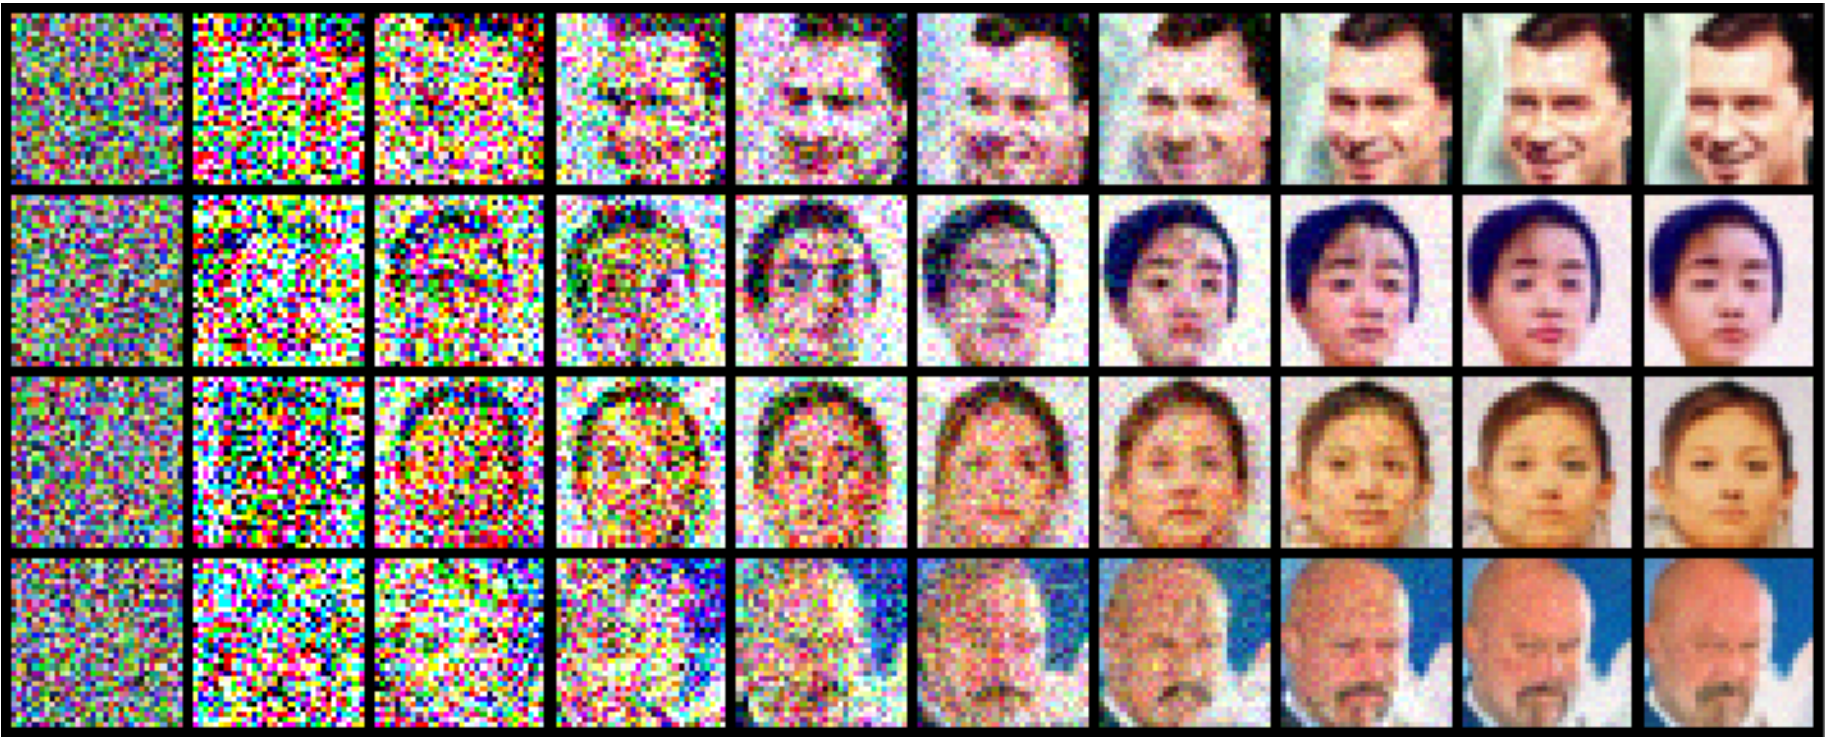
\includegraphics[width=0.9\linewidth]{figs/ald}
	\end{figure}
	\myfootnotewithlink{https://arxiv.org/abs/2006.09011}{Song Y. et al. Improved Techniques for Training Score-Based Generative Models, 2020}
\end{frame}
%=======
\section{DDPM vs NCSN}
%=======
\begin{frame}{DDPM vs NCSN}
	\begin{block}{NCSN objective}
		\vspace{-0.2cm}
		\[
			{\color{olive}\bbE_{p(\bx' | \bx, \sigma_l)}}\bigl\| {\color{teal}\bs_{\btheta}(\bx', \sigma_l)} - {\color{violet}\nabla_{\bx'} \log p(\bx' | \bx, \sigma_l)} \bigr\|^2_2 \rightarrow \min_{\btheta}
		\]
	\end{block}
	\vspace{-0.3cm}
	\begin{block}{DDPM objective}
		\vspace{-0.2cm}
		\[
			\cL_t = {\color{olive}\bbE_{\bepsilon \sim \cN(0, \bI)}} \left[ \frac{(1 - \alpha_t)^2}{2\tilde{\beta}_t \alpha_t} \left\| {\color{violet}\frac{\bepsilon}{\sqrt{1 - \bar{\alpha}_t}}} - {\color{teal}\frac{\bepsilon_{\btheta}(\bx_t, t)}{\sqrt{1 - \bar{\alpha}_t}}}\right\|^2 \right]
		\]
		\vspace{-0.7cm}
	\end{block}
	\begin{align*}
		q(\bx_t | \bx_0) &= \cN(\bx_t | \sqrt{\bar{\alpha}_t} \cdot \bx_0, (1 - \bar{\alpha}_t) \cdot \bI) \\
		{\color{violet}\nabla_{\bx_t} \log q(\bx_t | \bx_0)} &= - \frac{\bx_t - \sqrt{\bar{\alpha}_t} \cdot \bx_0}{1 - \bar{\alpha}_t} = - \frac{\bepsilon}{\sqrt{1 - \bar{\alpha}_t}}.
	\end{align*}
		Let reparametrize our model: 
		\vspace{-0.2cm}
		\[
			{\color{teal}\bs_{\btheta}(\bx_t, t)} = - \frac{\bepsilon_{\btheta}(\bx_t, t)}{\sqrt{1 - \bar{\alpha}_t}}.
		\]
	\myfootnotewithlink{https://arxiv.org/abs/2006.11239}{Ho J. Denoising Diffusion Probabilistic Models, 2020}
	\end{frame}
%=======
\begin{frame}{Summary}
	\begin{itemize}
		\item Score matching proposes to minimize Fisher divergence to get score function.
		\vfill
		\item Implicit score matching tries to avoid the value of original distribution $\pi(\bx)$. Sliced score matching makes implicit score matching scalable. 
		\vfill
		\item Denoising score matching minimizes Fisher divergence on noisy samples.		
		\vfill
		\item Noise conditioned score network uses multiple noise levels and annealed Langevin dynamics to fit score function.
		\vfill
		\item Objective of DDPM is closely related to the noise conditioned score network and score matching.	
	\end{itemize}
\end{frame}
\end{document} 